\chapter[Instalação do WSO2 ESB]{Instalação do WSO2 ESB}
"Este capítulo tem como objetivo apresentar o referencial teórico que embasa a pesquisa deste trabalho, incluindo conceitos abordados"

\section{Introdução}
Este manual de instalação é referente à ferramenta WSO2 ESB - WSO2 Enterprise Service Bus. Esta é uma das várias ferramentas que implementam o ESB, um mecanismo utilizado dentro da arquitetura SOA que possibilita a comunicação entre diversas aplicações utilizando diferentes formatos e protocolos de mensagens. Utilizando o ESB, uma aplicação se comunica apenas com esta ferramenta e esta, por sua vez, é responsável por transformar e entregar as mensagens do serviço destinatário correto (\cite{tutorial_ESB}).

\section{Pré-requisitos}
Para a instalação do WSO2 ESB, são necessários:
\begin{itemize}
\item JDK 1.6.* ou versão mais recente.
\item Variável de ambiente JAVA\_HOME configurada para <JDK\_HOME>.
\end{itemize}

\section{Instalação}
Os passos para a instalação do WSO2 ESB (versão 4.9.0) estão descritos abaixo:
\begin{enumerate}
\item Fazer o download do arquivo \textbf{wso2esb-4.9.0.zip}.
\item Extrair o arquivo \textbf{wso2esb-4.9.0.zip}.
\item No local onde o arquivo \textbf{wso2esb-4.9.0.zip} foi extraído (referenciado como <WSO2>), acessar a pasta <WSO2>\textbackslash bin.
\item Iniciar o servidor ESB executando:
\begin{itemize}
\item Em ambiente Linux: \textbf{wso2server.sh}
\item Em ambiente Windows: \textbf{wso2server.bat}
\end{itemize}
\end{enumerate}

O servidor estará completamente ativado quando a mensagem destacada abaixo
aparecer no \textit{log} da aplicação.

\begin{figure}[htb]
\centering
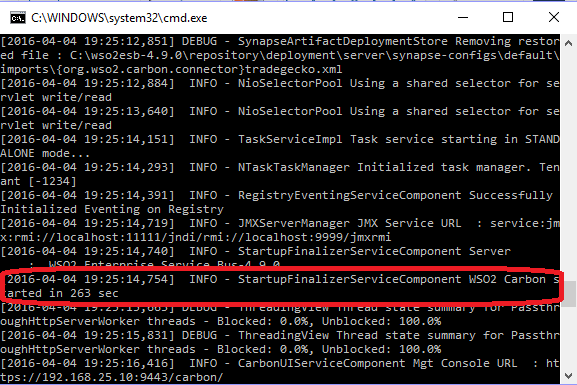
\includegraphics[width=1.0\textwidth]{figuras/log_iniciacao_wso2.PNG}
\caption{\textit{Log} de inicialização do servidor ESB.}
\label{log_iniciacao_wso2}
\end{figure}

\subsection{Trocando senha de acesso padrão}

Para a troca da senha padrão, basta acessar a aplicação ESB usando login e senha
padrão e, em seguida, acessar o menu conforme exibido na figura abaixo:

\begin{figure}[htb]
\centering
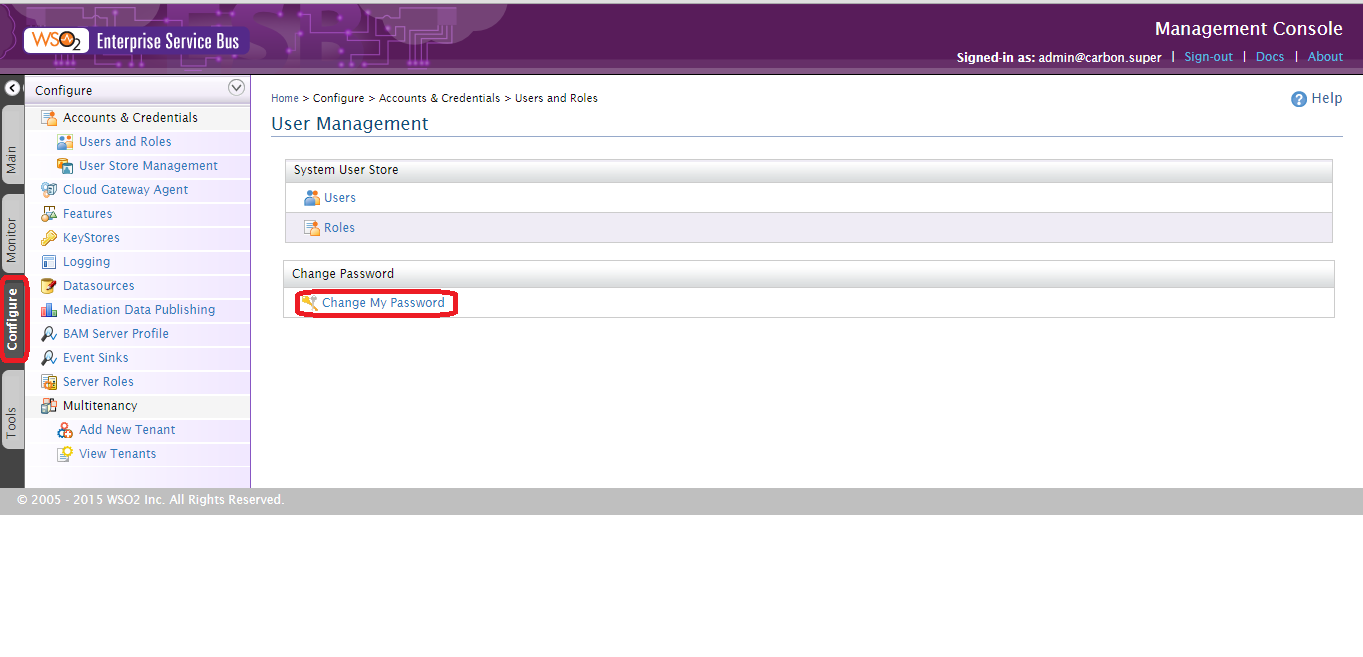
\includegraphics[width=1.0\textwidth]{figuras/mudar_senha.PNG}
\caption{Menu para troca de senha padrão.}
\label{mudar_senha}
\end{figure}